\genHeader
\fancyfoot[RO]{ $\triangleright$ \hyperlink{installEA vis}{Next visual task} \\ $\triangleright$ \hyperlink{simpleDemo common}{Next textual step} }

\subsection{Install our plugin for Eclipse}
 
 \vspace{0.5cm}
 
\begin{itemize}
\item[$\blacktriangleright$] Download\hypertarget{installPlugin common}{} and install Eclipse for modelling, ``Eclipse Modeling Tools (includes incubating
components)''\footnote{Please note that you \emph{have to} install \emph{Eclipse Modeling Tools}, from the Juno download packages, or nothing will work.  Do not
choose a different Eclipse package!  Although different versions might work, eMoflon is currently tested for Eclipse Juno and Java 1.7.} from
\url{http://www.eclipse.org/downloads/packages/release/juno/sr2} (Fig.~\ref{fig_downloadModelingPackage}).

\vspace{1.5cm}

\begin{figure}[htbp]
	\centering
  	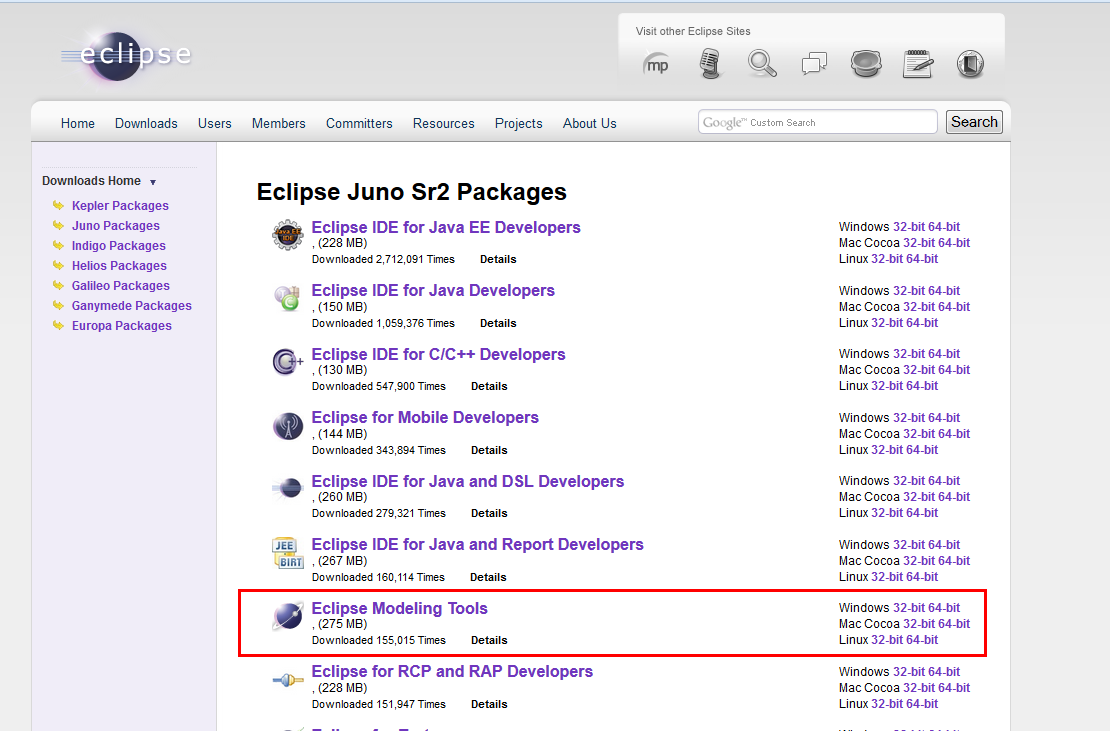
\includegraphics[width=0.86\textwidth]{eclipse_modelingTools}
	\caption{Download `Eclipse Modeling Tools'}
	\label{fig_downloadModelingPackage}
\end{figure}

\vspace{1cm}

\item[$\blacktriangleright$] Install our Eclipse Plugin from the following update site\footnote{For a detailed tutorial on how to install Eclipse and Eclipse
Plugins please refer to \url{http://www.vogella.de/articles/Eclipse/article.html}} \footnote{Please note: Calculating requirements and dependencies when
installing the plugin might take quite a while depending on your internet connection.}:
\url{http://www.moflon.org/fileadmin/download/moflon-ide/eclipse-plugin/update-site2}

\end{itemize}
